\documentclass[a4paper,11pt]{article}
\usepackage[margin=2.5cm]{geometry}
\usepackage{graphicx,url}
\title{Violet Creative Solutions\\Review of existing websites}
\author{Jovan Milicevic}
\date{24 November 2026}
\begin{document}
\maketitle
\section*{Introduction}
Violet Creative Solutions is an art studio. A client asking for a commission may find it easier to point to a piece they like than to describe a style from scratch. I looked at three websites to decide how to present our services, show examples of our work and use those examples in a commission request.
\section*{ArtStation}
ArtStation lets artists organise their work into albums and add several images or videos to one project page~\cite{art}. I liked being able to see the first sketch alongside the finished illustration. The artist profiles also cover software and work experience, which is more detail than a client usually needs when choosing a piece. For Violet, I would keep the sketch and finished work together and label the project with the service it belongs to.
\begin{center}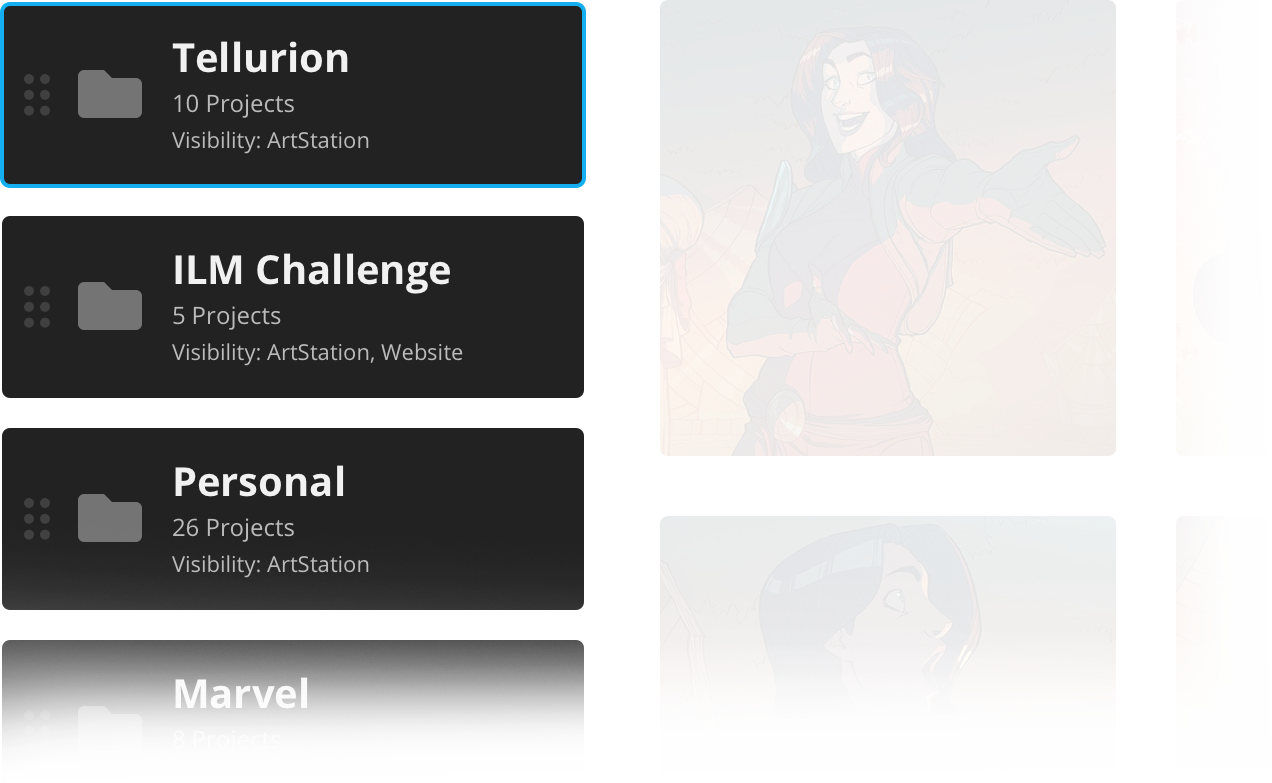
\includegraphics[width=.9\linewidth,height=.32\textheight,keepaspectratio]{artstation.png}\\Figure 1. Project albums and artwork on ArtStation (art by Matt Rhodes).\end{center}
\clearpage
\section*{Pinterest}
On Pinterest, visitors can search for images and save them to boards~\cite{pin}. A board gives a client a way to show the style they have in mind. The part it leaves unclear is what they like about a particular image. It might be the colours, the pose or both. On our site, a client could select a piece from the portfolio and explain that choice in the commission form.
\begin{center}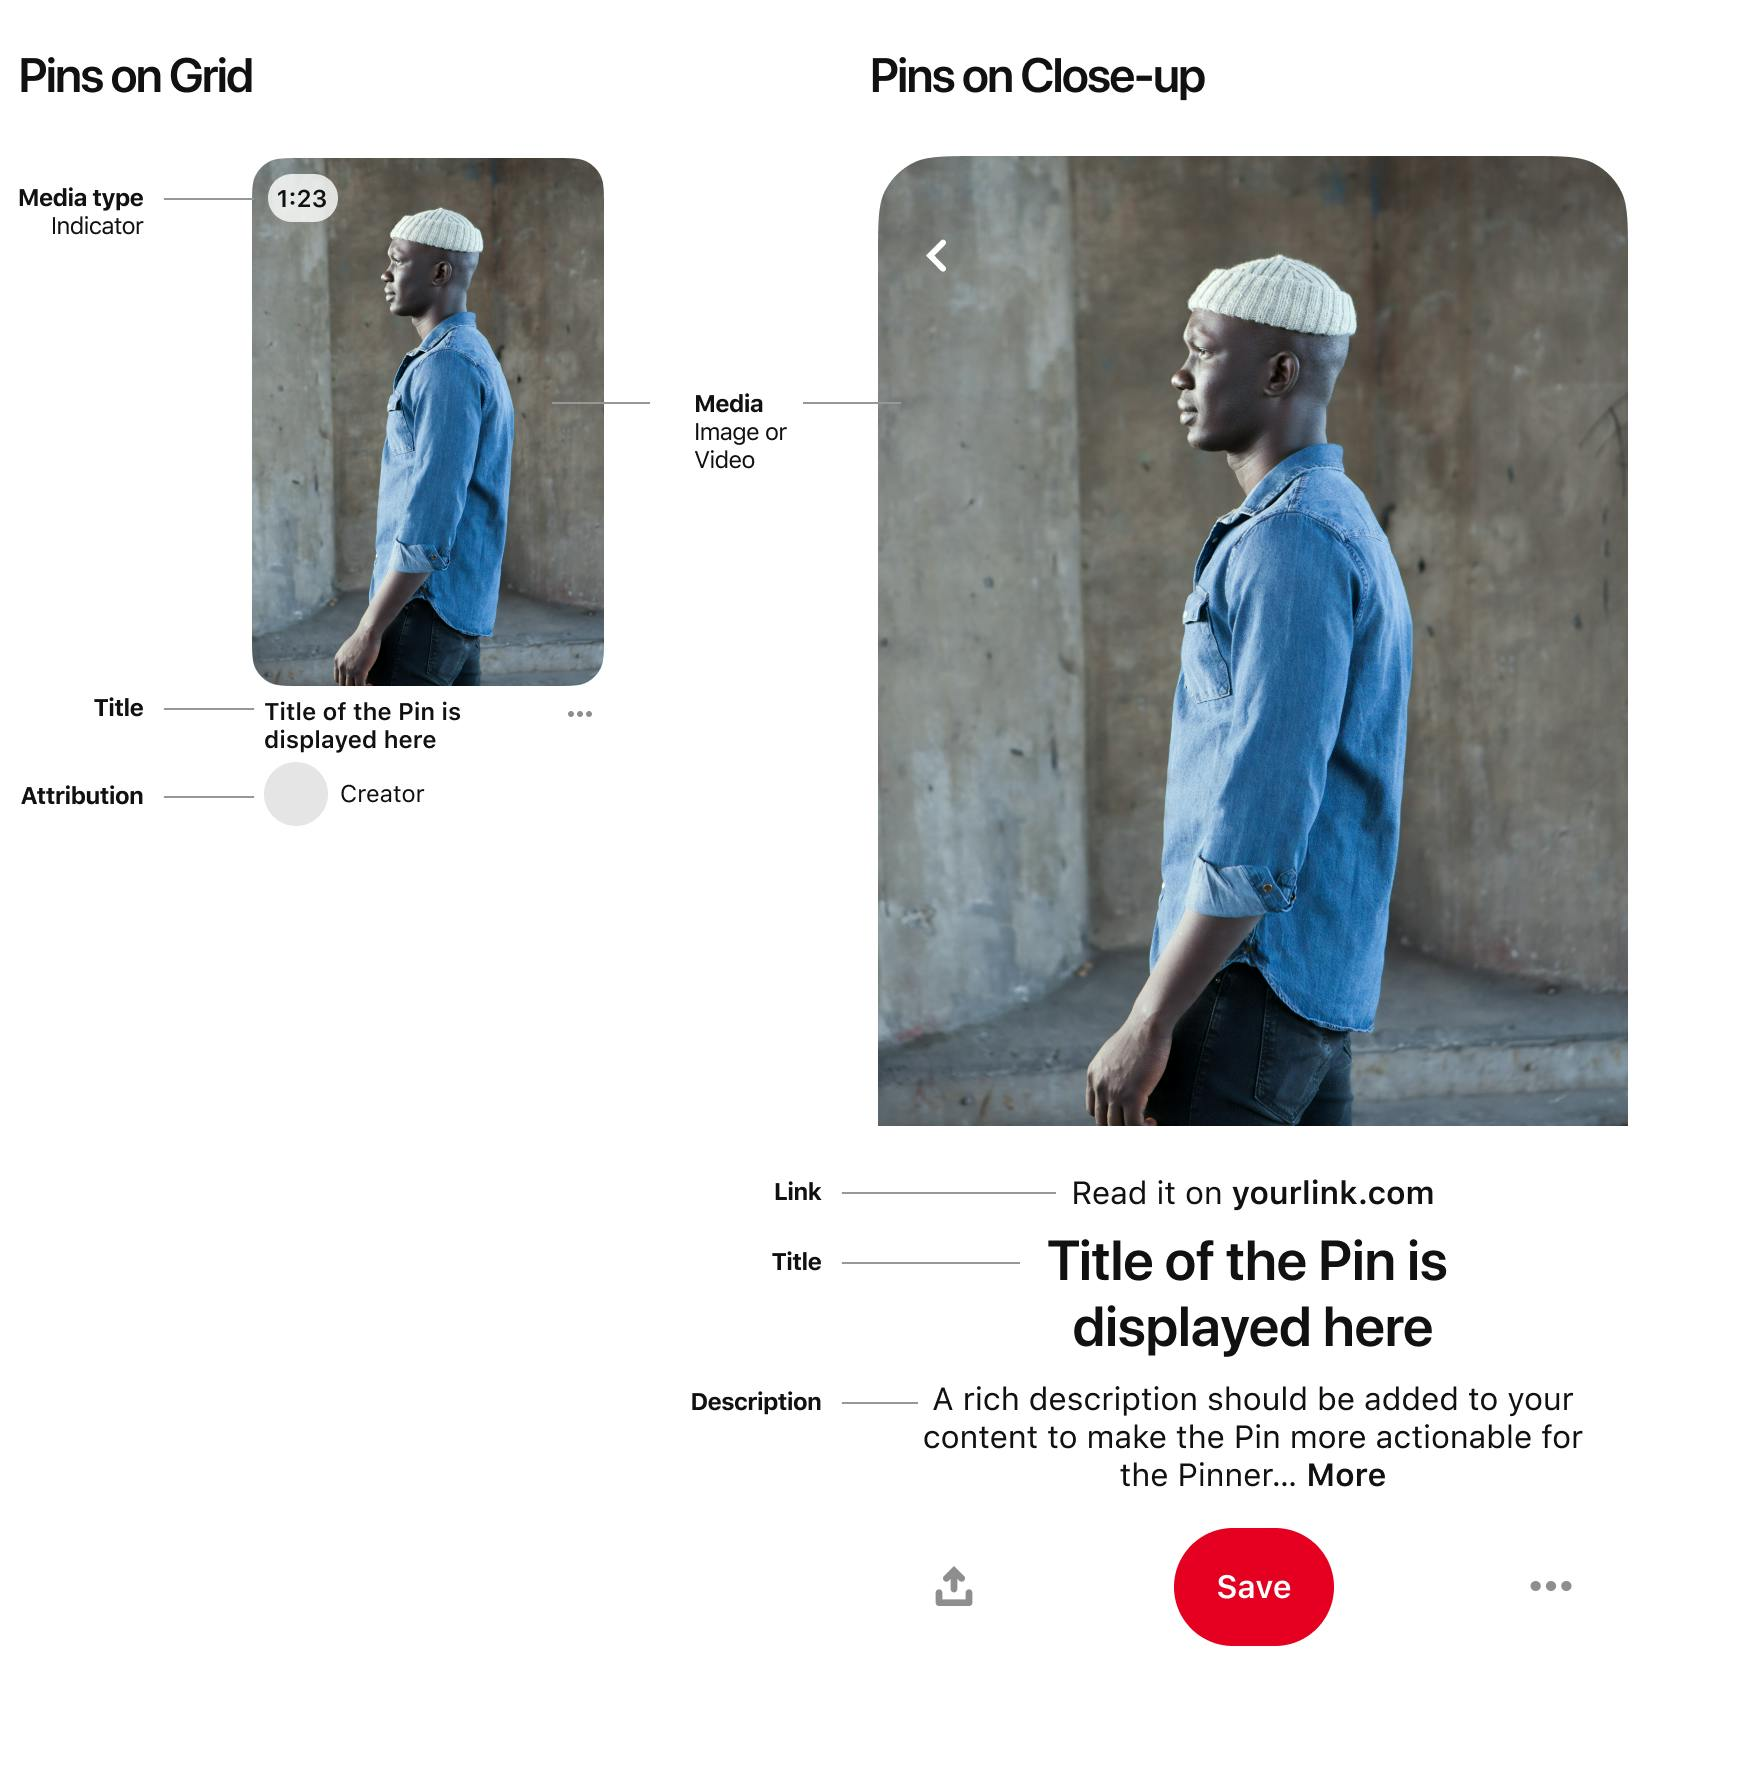
\includegraphics[width=.9\linewidth,height=.25\textheight,keepaspectratio]{pinterest.png}\\Figure 2. The same Pin in the grid and opened with the Save button.\end{center}
\section*{Microsoft}
I chose Microsoft for the layout of its home page. Visitors can choose Personal or Business at the top. Further down, each featured product has an image, a short description and a link~\cite{ms}. The cards make it easy to compare options, although the offers start to look similar after several rows. Violet only has four services, so I would keep them in one row. Selecting Living Ink, for example, would open the character art section of the portfolio.
\begin{center}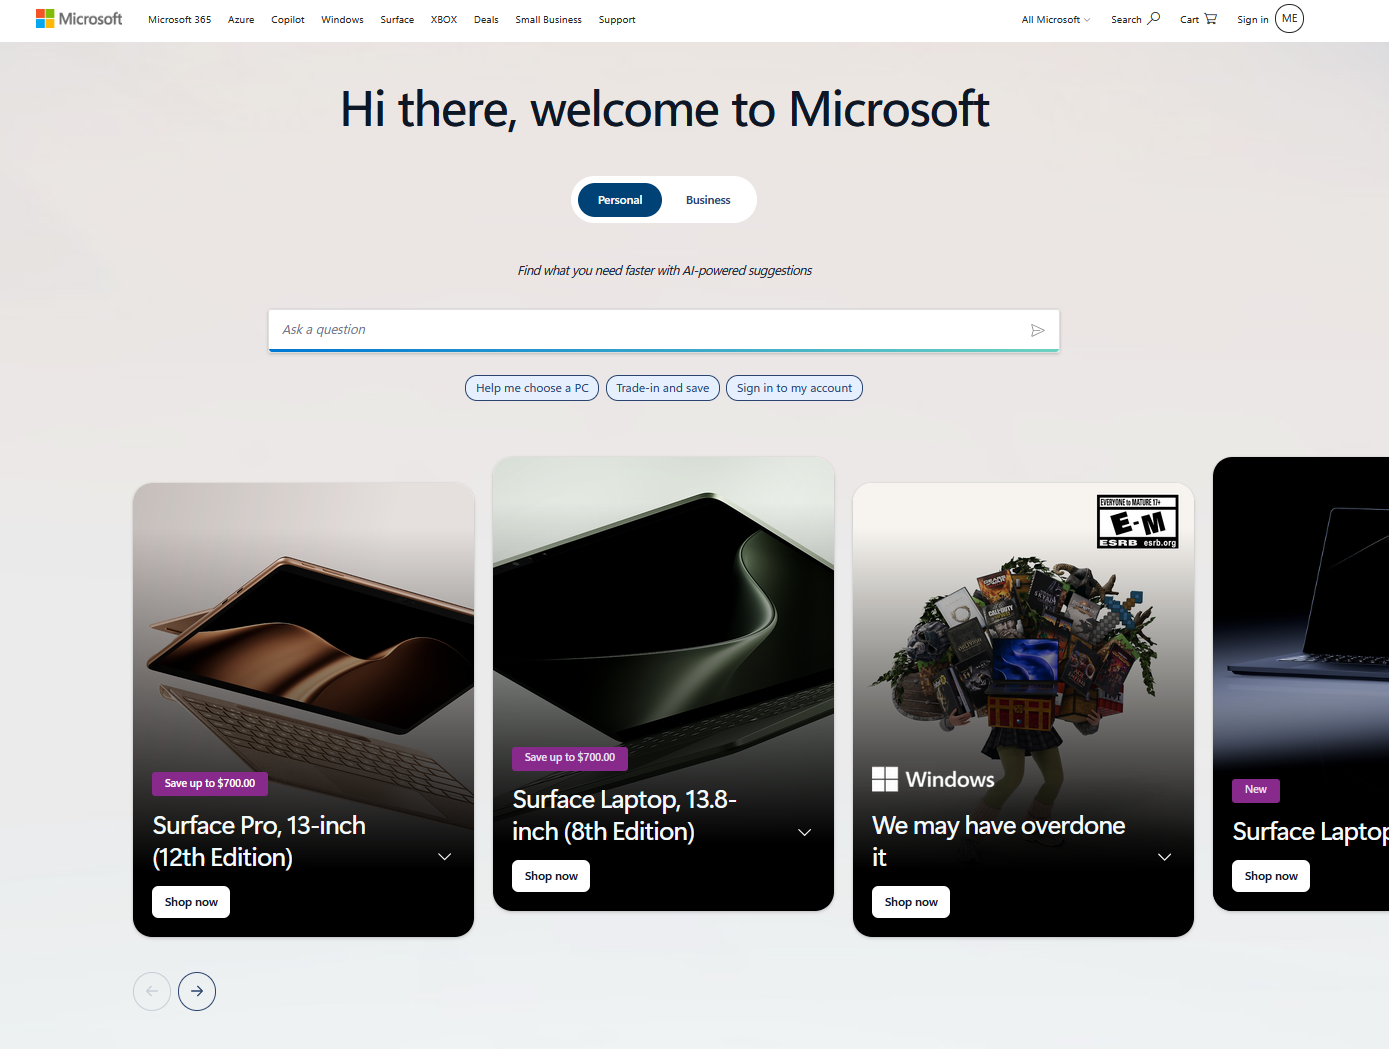
\includegraphics[width=.9\linewidth,height=.25\textheight,keepaspectratio]{microsoft.png}\\Figure 3. Personal, Business and the shortcuts on Microsoft's home page.\end{center}
\clearpage
\section*{Conclusion}
For Violet, I would use Microsoft's cards to introduce the four services and ArtStation's project layout to show how a piece developed. I would adapt Pinterest's idea of saving a reference by connecting it directly to the request. A client could open Living Ink, compare a sketch with the finished illustration and select \emph{Use as reference}. The form would already show the chosen piece, leaving the client to describe their own idea and add a reply email.
\begin{thebibliography}{9}
\bibitem{art} ArtStation, Portfolio. \url{https://www.artstation.com/about/artists/portfolio}
\bibitem{pin} Pinterest, All about Pinterest. \url{https://help.pinterest.com/en/guide/all-about-pinterest}
\bibitem{ms} Microsoft, Home page. \url{https://www.microsoft.com/en-us/}
\end{thebibliography}
\end{document}
